\documentclass[9pt, aspectratio=169]{beamer}
\usepackage{FiraSans}
\usetheme[subsectionpage=progressbar]{metropolis}
\usepackage[utf8]{inputenc}
\usepackage{amsmath}
\usepackage{amsfonts}
\usepackage{amssymb}
\usepackage{multicol}
\usepackage{tikz}
\usepackage{caption}
\usepackage{xcolor}
\usepackage[T1]{fontenc} 
\usepackage[skins]{tcolorbox}
\author{Nicola Roman\`o - nicola.romano@ed.ac.uk}
\title{Introduction to Version Control}
\setlength{\fboxsep}{0pt}
\setbeamertemplate {footline}{}

% Remove "Figure" in front of captions
% See https://tex.stackexchange.com/questions/82456/how-to-remove-figure-caption-prefix-figure-in-beamer
\captionsetup{labelformat=empty,labelsep=none}

\titlegraphic{\centering \includegraphics[scale=.5]{instituteLogo.png}}
\date{}

\begin{document}

\newtcolorbox{codebox}{enhanced,
    top=2pt,
    left=2pt,
    right=2pt,
    bottom=2pt,
    boxrule=0pt,
    leftrule=5pt,
    sharp corners,
    colback=gray!20,
    colframe=blue!60!black}

\begin{frame}
    \titlepage
\end{frame}

\begin{frame}
    {Importance of Code Versioning}
    \begin{columns}[T]
        \begin{column}{.5\textwidth}
            \begin{itemize}
                \item When writing code you often change files multiple times.
                \item It's tempting to keep multiple copies of the same file with different names, for example to keep track of different versions before and after a change.
                \item This can lead to confusion and errors.
            \end{itemize}
            \includegraphics[width=\textwidth]{messy_filenames.png}
        \end{column}
        \pause
        \begin{column}{.5\textwidth}
            \begin{itemize}
                \item A version control system keeps track of changes and allows you to go back to previous versions.
                \item It also enables collaboration and sharing of code with others.
            \end{itemize}
            \centering
            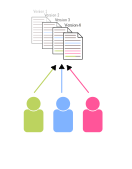
\includegraphics[width=.7\textwidth]{version_control.png}
        \end{column}
    \end{columns}
\end{frame}

\begin{frame}{Git and GitHub}
    Today we are going to talk about two tools for version control:

    \begin{itemize}
        \item GitHub is a platform for hosting code repositories and collaborating on projects.
        \item It uses Git, a version control system, to track changes to code over time.
        \item Enables collaboration by allowing multiple people to contribute to the same project.
    \end{itemize}
    \begin{center}
        \includegraphics[width=0.7\textwidth]{git-github-logo.png}
    \end{center}
\end{frame}

\begin{frame}{What is Git?}
    \begin{itemize}
        \item Git is a version control system that lets you track changes in your project.
        \item It creates snapshots of your project over time.
        \item You can use Git locally to manage versions, and then use GitHub to share and collaborate.
    \end{itemize}
\end{frame}

\section{Setting Up your system}

\begin{frame}{Installing Git and registering on GitHub}
    \begin{columns}[T]
        \begin{column}{.4\textwidth}
            \centering
            https://git-scm.com/\\
            \includegraphics[width=.4\textwidth]{git-logo.png}
            \includegraphics[width=.4\textwidth]{git_qr.png}\\
            \vspace{1em}
            https://www.github.com/\\
            \includegraphics[width=.4\textwidth]{github_logo.png}
            \includegraphics[width=.4\textwidth]{github_qr.png}
        \end{column}
        \pause
        \begin{column}{.6\textwidth}
            \centering
            Check GIT installation\\
            \vspace{1em}
            \includegraphics[width=\textwidth]{git_version.png}
            Configure GIT\\
            \includegraphics[width=\textwidth]{git_config.png}
        \end{column}
    \end{columns}
\end{frame}

\begin{frame}
    {Some Git nomencalture}
    When using Git, you will encounter some terms that are important to understand:

    \begin{itemize}
        \item \textbf{Repository}: a directory that contains your project, including the files/directories in your project, as well as the history of changes to those files.
        \pause
        \item \textbf{Staging}: the process of preparing files to be committed. This is done before you commit changes to your repository.
        \item \textbf{Commit}: a snapshot of your project at a specific point in time.
        \item \textbf{Push}: sending your changes from the local computer to a remote repository.
        \item \textbf{Pull}: getting changes from a remote repository to your local computer.
        \pause        
        \item \textbf{Branch}: a parallel version of your repository that allows you to work on a feature or bugfix without affecting the main project.
        \item \textbf{Pull request}: a request to merge changes from one branch to another.
    \end{itemize}

\end{frame}


\begin{frame}
    {Summary of git commands}
    \centering
    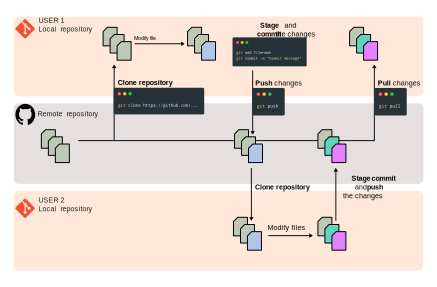
\includegraphics[width=.91\textwidth]{git workflow.png}
\end{frame}
\end{document}

